% Dit werk is gelicenseerd onder de licentie Creative Commons Naamsvermelding-GelijkDelen 4.0 Internationaal. Ga naar http://creativecommons.org/licenses/by-sa/4.0/ om een kopie van de licentie te kunnen lezen.
\documentclass[t]{beamer}

% vaak gebruikte packages, nederlands


\usepackage{a4wide}                     % Iets meer tekst op een bladzijde
\usepackage[dutch]{babel}               % Voor nederlandstalige hyphenatie (woordsplitsing)
%\usepackage{amsmath,amsthm}             % Uitgebreide wiskundige mogelijkheden
%\usepackage{amssymb}                    % Voor speciale symbolen zoals de verzameling Z, R...
%\usepackage{makeidx}                    % Om een index te maken
\usepackage{url}                        % Om url's te verwerken
\usepackage{graphicx,subfigure}         % Om figuren te kunnen verwerken
\usepackage{color}
\usepackage{multicol}
\usepackage[small,bf,hang]{caption}     % Om de captions wat te verbeteren
%\usepackage{xspace}                     % Magische spaties na een commando
\usepackage[latin1]{inputenc}           % Om niet ascii karakters rechtstreeks te kunnen typen
\usepackage{float}                      % Om nieuwe float environments aan te maken. Ook optie H!
\usepackage{flafter}                    % Opdat floats niet zouden voorsteken
\usepackage[section]{placeins}			% Om ervoor te zorgen dat floats binnen dezelfde section blijven
%\usepackage{listings}                   % Voor het weergeven van letterlijke text en codelistings
%\usepackage[numbers]{natbib}            % Voor juiste citatie stijl
\usepackage[nottoc]{tocbibind}			% Bibliografie en inhoudsopgave in ToC; zie tocbibind.dvi
\usepackage{eurosym}                    % om het euro symbool te krijgen
\usepackage{textcomp}                   % Voor onder andere graden celsius
\usepackage{fancyhdr}                   % Voor fancy headers en footers
\usepackage[Gray,squaren,thinqspace,thinspace]{SIunits} % Om elegant eenheden te zetten
\usepackage[version=3]{mhchem}          % Voor elegante scheikundige formules
%\usepackage{emptypage}					% Om de lege pagina's voor een hoofdstuk mooi te maken
\usepackage{thmtools}                   % theorem tools
\usepackage{collect}
\usepackage{parskip}                    % Om paragrafen met een verticale spatie ipv horizontaal te laten beginnen



\usepackage[plainpages=false]{hyperref}    % Om hyperlinks te hebben in het pdfdocument.



%%%%%%%%%%%%%%%%%%%%%%%%%%%%%%
% Algemene instellingen van het document.
%%%%%%%%%%%%%%%%%%%%%%%%%%%%%%

%\setlength{\parindent}{0cm}             % Inspringen van eerste lijn van paragrafen is niet gewenst.
%\setlength{\parskip}{0cm}
\renewcommand{\baselinestretch}{1.2} 	% De interlinie afstand wat vergroten.

\setcounter{MaxMatrixCols}{50}          % Max 20 kolommen in een matrix

% Vandaar dat we expliciet aangeven wanneer we wensen dat een nieuwe paragraaf begint:
% \par zorgt ervoor dat er een nieuwe paragraaf begint en
% \vspace zorgt voor verticale ruimte.
\newcommand{\npar}{}



%%%%%%%%%%%%%%%%%%%%%%%%%%%%%%
% Nieuwe omgevingen
%%%%%%%%%%%%%%%%%%%%%%%%%%%%%%

% Een definitie omgeving zonder nummering voor definities
%\newtheoremstyle{definitie_style}{}{}{\itshape}{}{\bfseries}{}{ }{}
%\theoremstyle{definitie_style}
%\newtheorem*{definitie}{}


    
%%%%%%%%%%%%%%%%%%%%%%%%%%%%%%
% Nieuwe commandos
%%%%%%%%%%%%%%%%%%%%%%%%%%%%%%

% De differentiaal operator
\newcommand{\diff}{\ensuremath{\mathrm{d}}}
\newcommand{\subsdiff}{\ensuremath{\mathrm{D}}}
\newcommand{\vardiff}{\ensuremath{\mathrm{\delta}}}

% Super en subscript
\newcommand{\supsc}[1]{\ensuremath{^{\text{#1}}}}   % Superscript in tekst
\newcommand{\subsc}[1]{\ensuremath{_{\text{#1}}}}   % Subscript in tekst

% Vectoren en matrices
\newcommand{\vt}[1]{\ensuremath{\boldsymbol{#1}}} % vector in juiste lettertype
\newcommand{\mx}[1]{\ensuremath{\mathsf{#1}}}	  % matrix in juiste lettertype

% Nieuw commando om iets te benadrukken en tegelijkertijd in de index te steken.
\newcommand{\begrip}[1]{\index{#1}\textbf{#1}\xspace}

% Graden celcius
\newcommand{\degC}{\ensuremath{^\circ \mathrm{C}}}


% nieuw commando om svg files dynamisch te updaten
\newcommand{\executeiffilenewer}[3]{%
\ifnum\pdfstrcmp{\pdffilemoddate{#1}}%
{\pdffilemoddate{#2}}>0%
{\immediate\write18{#3}}\fi%
}
% nieuw commando om. svg figuren in te voegen
% Gebruik: \includesvg{path/filename.svg}
\newcommand{\includesvg}[2][0]{%
\executeiffilenewer{#2.svg}{#2.pdf}%
{inkscape -z -C --file=#2.svg %
--export-pdf=#2.pdf --export-latex}%
\ifx#10
	\let\svgwidth\undefined
\else
	\def\svgwidth{#1}
\fi%
\input{#2.pdf_tex}%
\ifx \svgwidth\undefined
\else
	\let\svgwidth\undefined
\fi%
}

% nieuw commando om .fig figuren in te voegen
\newcommand{\includefig}[2][0]{%
\ifx#10
	\let\figwidth\undefined
\else
	\def\figwidth{#1}
\fi%
\input{#2.pdf_tex}%
\ifx \figwidth\undefined
\else
	\let\figwidth\undefined
\fi%
}

\input{tex/packages_slides}

\subtitle{Leidingstelsels}

\begin{document}

	\frame{\titlepage}
%%%%%%%%%%%%%%%%%%%%%%%%%%%%%%%%%%%%%%%%%%%%%%%%%%%%%%%%%%%%%%%%%%%%%%%%%%%
	\section{Inleiding}
	\begin{frame}
		\frametitle{Voorbeeld}
		\center
    	\includegraphics[width=\textwidth]{fig/stroming_in_leidingen/Richard-Steinberg-The-Pipeline-Blog-51.jpg}\\
    	\footnotesize{Bron: http://www.etftrends.com/}
  	\end{frame}
%%%%%%%%%%%%%%%%%%%%%%%%%%%%%%%%%%%%%%%%%%%%%%%%%%%%%%%%%%%%%%%%%%%%%%%%%%%
  	\section{Mechanische energie}
  	\begin{frame}
		\frametitle{Bernoulli}
		\only<1-4>{
			Behoud van mechanisch energie:
			\begin{equation*}
				p_2 + \rho \frac{1}{2} v_2^2 + \rho g z_2 = p_1 + \rho \frac{1}{2} v_1^2 + \rho g z_1
			\end{equation*}
		}
		\only<2-4>{
			Door viskeuze wrijving wordt een gedeelte van de mechanische energie gedissipeerd:
			\begin{equation*}
				p_2 + \rho \frac{1}{2} v_2^2 + \rho g z_2 = p_1 + \rho \frac{1}{2} v_1^2 + \rho g z_1 - \Delta E
			\end{equation*}
		}
		\only<3-4>{
			Voor een rechte horizontale cilindrische leiding:
			\begin{equation*}
				\Delta E = p_1 - p_2  
			\end{equation*}	
		}
		\only<4-4>{
			\begin{equation*}
				\Delta E = f \frac{1}{2} \rho v^2 \frac{L}{D}
			\end{equation*}
		}
	\end{frame}
%%%%%%%%%%%%%%%%%%%%%%%%%%%%%%%%%%%%%%%%%%%%%%%%%%%%%%%%%%%%%%%%%%%%%%%%%%%
  	\begin{frame}
		\frametitle{Ladingsverlies}
		\only<1-3>{
			Stel de vergelijking voor mechanische energie voor in eenheid hoogte:
			\begin{equation}
				\frac{p_2}{\rho g} + \frac{v_2^2}{2 g} + z_2 = \frac{p_1}{\rho g} + \frac{v_1^2}{2 g} + z_1 - h_L
			\end{equation}		
		}
		\only<2-3>{
			Ladingsverlies voor een cilindrische leiding:
			\begin{equation}
				h_\mathrm{L} = f \frac{v^2}{2 g} \frac{L}{D}
			\end{equation}
		}
		\only<3-3>{
			\begin{equation}
				h_\mathrm{L} = 8 f \frac{\dot{V}^2}{g \pi^2} \frac{L}{D^5}
			\end{equation}
		}
	\end{frame}
%%%%%%%%%%%%%%%%%%%%%%%%%%%%%%%%%%%%%%%%%%%%%%%%%%%%%%%%%%%%%%%%%%%%%%%%%%%
  	\begin{frame}
		\frametitle{Grafische voorstelling}
		
	\end{frame}
%%%%%%%%%%%%%%%%%%%%%%%%%%%%%%%%%%%%%%%%%%%%%%%%%%%%%%%%%%%%%%%%%%%%%%%%%%%
  	\section{Lokale ladingsverliezen}
  	\begin{frame}
		\frametitle{Voorbeelden}
		\center
		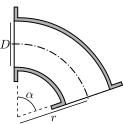
\includegraphics[width=0.3\textwidth]{fig/appendix/Bocht} \quad
		\includegraphics[width=0.3\textwidth]{fig/appendix/Gelijkdelijke_vernauwing} \quad
		\includegraphics[width=0.3\textwidth]{fig/appendix/Gelijkdelijke_verwijding}
		\\
		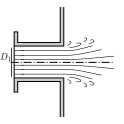
\includegraphics[width=0.3\textwidth]{fig/appendix/Uitstroming} \quad
		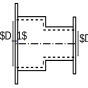
\includegraphics[width=0.3\textwidth]{fig/appendix/Vernauwing} \quad
		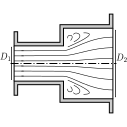
\includegraphics[width=0.3\textwidth]{fig/appendix/Verwijding}
	\end{frame}
%%%%%%%%%%%%%%%%%%%%%%%%%%%%%%%%%%%%%%%%%%%%%%%%%%%%%%%%%%%%%%%%%%%%%%%%%%%
  	\begin{frame}
		\frametitle{Verliescoëfficient}	
		\only<1-3>{
			\center
			Lokale ladings verliezen kunnen in rekening gebracht worden met behulp van een empirisch bepaalde verliescoëfficient $\zeta$
		}
		
		\only<2-3>{
			\begin{equation*}
				h_\mathrm{L,lokaal} = \zeta \frac{v^2}{2 g}
			\end{equation*}
		}
		\only<3-3>{
			\begin{equation*}
				h_\mathrm{L,lokaal} = \zeta \frac{\dot{V}^2}{2 g A^2}
			\end{equation*}
		}
		
	\end{frame}
%%%%%%%%%%%%%%%%%%%%%%%%%%%%%%%%%%%%%%%%%%%%%%%%%%%%%%%%%%%%%%%%%%%%%%%%%%%
  	\begin{frame}
		\frametitle{Plotse Verwijding}
		\only<1>{
			\center
			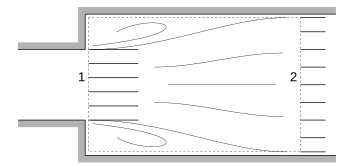
\includegraphics[width=\textwidth]{fig/leidingstelsels/Plotse_verwijding}
		}
		\only<2-5>{
			\begin{textblock}{5}(0,3)
            	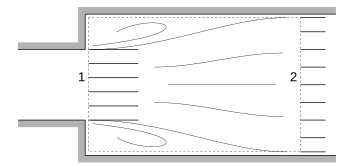
\includegraphics[width=5cm]{fig/leidingstelsels/Plotse_verwijding}
       		\end{textblock}
       		\vspace{2.5cm}
		}
		\only<2-5>{
			\begin{equation*}
				p_1 A_2 - p_2 A_2 = \rho A_2 v_2 (v_2-v_1)
			\end{equation*}
		}
		\only<3-5>{
			\begin{equation*}
				\frac{p_2}{\rho g} + \frac{v_2^2}{2 g} = \frac{p_1}{\rho g} + \frac{v_1^2}{2 g} - h_L
			\end{equation*}
		}
		\only<4-5>{
			\begin{equation*}
				h_L = \frac{v_1^2}{2 g} \left(1 - 2\frac{v_2}{v_1} + \frac{v_2^2}{v_1^2} \right)
			\end{equation*}
		}
		\only<5-5>{
			\begin{equation*}
				h_L = \frac{v_1^2}{2 g} \left(1 - \frac{A_1}{A_2} \right)^2
			\end{equation*}
		}
	\end{frame}
%%%%%%%%%%%%%%%%%%%%%%%%%%%%%%%%%%%%%%%%%%%%%%%%%%%%%%%%%%%%%%%%%%%%%%%%%%%
  	\begin{frame}
		\frametitle{Voorbeeld van empirische data}
		\center
		\begin{tabular}{p{7cm} p{3cm}}
			\vtop{\null\hbox{
				\begin{tabular}{l c c c c c}
					$r/D$        & 1    & 2    & 4    & 6    & 10   \\
					\hline
					$\zeta$ glad & 0.21 & 0.14 & 0.11 & 0.09 & 0.11 \\
					$\zeta$ ruw  & 0.51 & 0.30 & 0.23 & 0.18 & 0.20 \\
				\end{tabular}
			}}
			&
			\vtop{\null\hbox{
				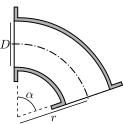
\includegraphics[width=3cm]{fig/appendix/Bocht}
			}}
		\end{tabular}
		
		\center
		Het totale ladingsverlies is steeds het lokale verlies plus het verlies ten gevolge van de lengte van de leiding.
	
	\end{frame}
%%%%%%%%%%%%%%%%%%%%%%%%%%%%%%%%%%%%%%%%%%%%%%%%%%%%%%%%%%%%%%%%%%%%%%%%%%%	
	\begin{frame}
		\frametitle{Voorbeelden}
		\center
		\includegraphics[height=0.8\textheight]{fig/appendix/verwijding}
	\end{frame}
%%%%%%%%%%%%%%%%%%%%%%%%%%%%%%%%%%%%%%%%%%%%%%%%%%%%%%%%%%%%%%%%%%%%%%%%%%%	
	\begin{frame}
		\frametitle{Voorbeelden}
		\center
		\includegraphics[height=0.8\textheight]{fig/appendix/gelijkdelijke_verwijding}
	\end{frame}
%%%%%%%%%%%%%%%%%%%%%%%%%%%%%%%%%%%%%%%%%%%%%%%%%%%%%%%%%%%%%%%%%%%%%%%%%%%	
	\begin{frame}
		\frametitle{Voorbeelden}
		\center
		\includegraphics[height=0.8\textheight]{fig/appendix/uitstroming}
	\end{frame}
%%%%%%%%%%%%%%%%%%%%%%%%%%%%%%%%%%%%%%%%%%%%%%%%%%%%%%%%%%%%%%%%%%%%%%%%%%%	
	\begin{frame}
		\frametitle{Voorbeelden}
		\center
		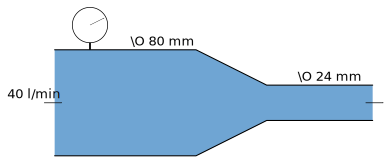
\includegraphics[height=0.8\textheight]{fig/appendix/vernauwing}
	\end{frame}
%%%%%%%%%%%%%%%%%%%%%%%%%%%%%%%%%%%%%%%%%%%%%%%%%%%%%%%%%%%%%%%%%%%%%%%%%%%	
	\begin{frame}
		\frametitle{Voorbeelden}
		\center
		\includegraphics[height=0.8\textheight]{fig/appendix/gelijkdelijke_vernauwing}
	\end{frame}	
%%%%%%%%%%%%%%%%%%%%%%%%%%%%%%%%%%%%%%%%%%%%%%%%%%%%%%%%%%%%%%%%%%%%%%%%%%%	
	\begin{frame}
		\frametitle{Voorbeelden}
		\center
		\includegraphics[height=0.8\textheight]{fig/appendix/instroming}
	\end{frame}	
%%%%%%%%%%%%%%%%%%%%%%%%%%%%%%%%%%%%%%%%%%%%%%%%%%%%%%%%%%%%%%%%%%%%%%%%%%%	
	\begin{frame}
		\frametitle{Voorbeelden}
		\center
		\includegraphics[height=0.8\textheight]{fig/appendix/afgeronde_instroming}
	\end{frame}	
%%%%%%%%%%%%%%%%%%%%%%%%%%%%%%%%%%%%%%%%%%%%%%%%%%%%%%%%%%%%%%%%%%%%%%%%%%%
  	\section{Serie en parallel schakeling}
  	\begin{frame}
		\frametitle{Serieschakeling}
		\only<1-3>{
			\center
			\includegraphics[width=0.8\textwidth]{fig/leidingstelsels/serieschakeling}
		}
		\only<2-3>{	
			\begin{align*}
				\dot{V}_\mathrm{serie} &= \dot{V}_i \\
				h_\mathrm{L,serie} &= \sum h_\mathrm{L,i}
			\end{align*}
		}
		\only<3-3>{
			\center
			Het totale ladingsverlies in een serieschakeling van elementen is de som van de ladingsverliezen
		}
	\end{frame}
%%%%%%%%%%%%%%%%%%%%%%%%%%%%%%%%%%%%%%%%%%%%%%%%%%%%%%%%%%%%%%%%%%%%%%%%%%%
  	\begin{frame}
		\frametitle{Parallelschakeling}
		\only<1-3>{
			\center
			\includegraphics[width=0.8\textwidth]{fig/leidingstelsels/parallelschakeling}
		}
		\only<2-3>{	
			\begin{align*}
				\dot{V}_\mathrm{parallel} &= \sum \dot{V}_i \\
				h_\mathrm{L,parallel} &= h_\mathrm{L,i}
			\end{align*}
		}
		\only<3-3>{
			\center
			Het ladingsverlies in elke tak van een parallelschakeling is gelijk aan het totale ladingsverlies
		}
	\end{frame}
%%%%%%%%%%%%%%%%%%%%%%%%%%%%%%%%%%%%%%%%%%%%%%%%%%%%%%%%%%%%%%%%%%%%%%%%%%%
\end{document}